\documentclass{standalone}
\usepackage{tikz}
\usetikzlibrary{patterns, positioning}


\begin{document}
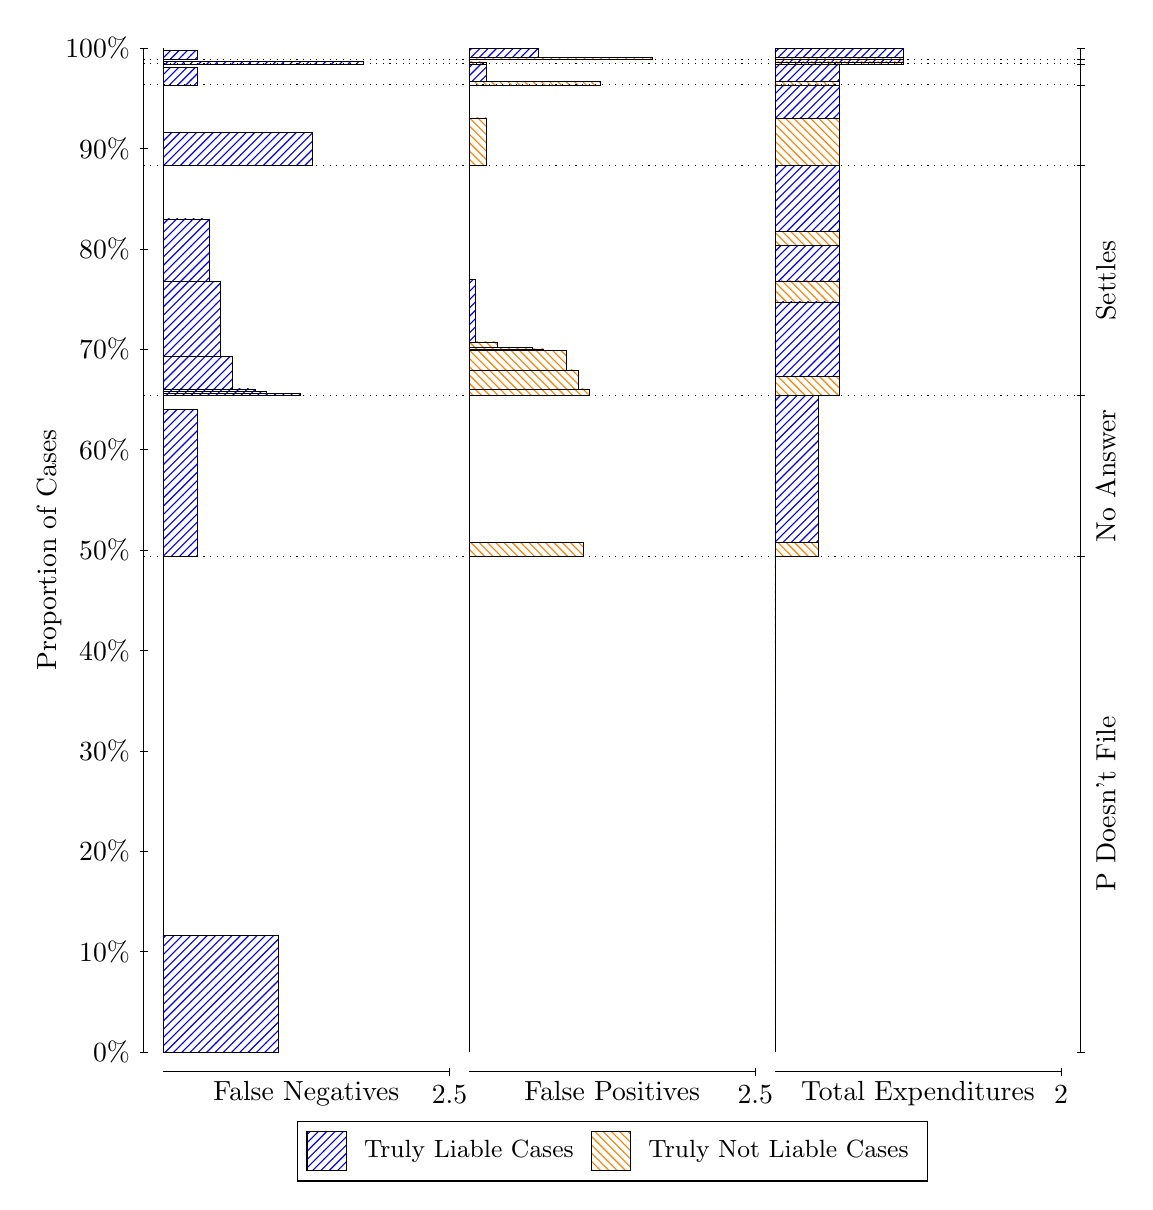
\begin{tikzpicture}
\draw[black, very thin] (1.5,1.75) -- (1.5,14.5);
\node[rotate=90, text=black, anchor=center] at (0.3, 8.125) {Proportion of Cases};
\draw[black, very thin] (1.45,1.75) -- (1.55,1.75);
\node[text=black, anchor=east] at (1.45, 1.75) {0\%};
\draw[black, very thin] (1.45,3.025) -- (1.55,3.025);
\node[text=black, anchor=east] at (1.45, 3.025) {10\%};
\draw[black, very thin] (1.45,4.3) -- (1.55,4.3);
\node[text=black, anchor=east] at (1.45, 4.3) {20\%};
\draw[black, very thin] (1.45,5.575) -- (1.55,5.575);
\node[text=black, anchor=east] at (1.45, 5.575) {30\%};
\draw[black, very thin] (1.45,6.85) -- (1.55,6.85);
\node[text=black, anchor=east] at (1.45, 6.85) {40\%};
\draw[black, very thin] (1.45,8.125) -- (1.55,8.125);
\node[text=black, anchor=east] at (1.45, 8.125) {50\%};
\draw[black, very thin] (1.45,9.4) -- (1.55,9.4);
\node[text=black, anchor=east] at (1.45, 9.4) {60\%};
\draw[black, very thin] (1.45,10.675) -- (1.55,10.675);
\node[text=black, anchor=east] at (1.45, 10.675) {70\%};
\draw[black, very thin] (1.45,11.95) -- (1.55,11.95);
\node[text=black, anchor=east] at (1.45, 11.95) {80\%};
\draw[black, very thin] (1.45,13.225) -- (1.55,13.225);
\node[text=black, anchor=east] at (1.45, 13.225) {90\%};
\draw[black, very thin] (1.45,14.5) -- (1.55,14.5);
\node[text=black, anchor=east] at (1.45, 14.5) {100\%};

\draw[black, very thin] (13.4,1.75) -- (13.4,14.5);
\draw[black, very thin] (13.35,1.75) -- (13.45,1.75);
\node[anchor=west] at (13.35, 1.75) {};
\draw[black, very thin] (13.35,8.0481) -- (13.45,8.0481);
\node[anchor=west] at (13.35, 8.0481) {};
\draw[black, very thin] (13.35,10.086) -- (13.45,10.086);
\node[anchor=west] at (13.35, 10.086) {};
\draw[black, very thin] (13.35,13.01) -- (13.45,13.01);
\node[anchor=west] at (13.35, 13.01) {};
\draw[black, very thin] (13.35,14.032) -- (13.45,14.032);
\node[anchor=west] at (13.35, 14.032) {};
\draw[black, very thin] (13.35,14.298) -- (13.45,14.298);
\node[anchor=west] at (13.35, 14.298) {};
\draw[black, very thin] (13.35,14.351) -- (13.45,14.351);
\node[anchor=west] at (13.35, 14.351) {};
\draw[black, very thin] (13.35,14.5) -- (13.45,14.5);
\node[anchor=west] at (13.35, 14.5) {};

\draw[black, very thin, pattern color=blue, pattern=north east lines] (1.75,1.75) rectangle (3.2033,3.2333);
\draw[black, very thin, pattern color=orange, pattern=north west lines] (1.75,3.2333) rectangle (1.75,8.0481);
\draw[black, very thin, pattern color=blue, pattern=north east lines] (1.75,8.0481) rectangle (2.186,9.9081);
\draw[black, very thin, pattern color=orange, pattern=north west lines] (1.75,9.9081) rectangle (1.75,10.086);
\draw[black, very thin, pattern color=blue, pattern=north east lines] (1.75,10.086) rectangle (3.494,10.114);
\draw[black, very thin, pattern color=blue, pattern=north east lines] (1.75,10.114) rectangle (3.058,10.135);
\draw[black, very thin, pattern color=blue, pattern=north east lines] (1.75,10.135) rectangle (2.9127,10.17);
\draw[black, very thin, pattern color=blue, pattern=north east lines] (1.75,10.17) rectangle (2.622,10.588);
\draw[black, very thin, pattern color=blue, pattern=north east lines] (1.75,10.588) rectangle (2.4767,11.537);
\draw[black, very thin, pattern color=blue, pattern=north east lines] (1.75,11.537) rectangle (2.3313,12.329);
\draw[black, very thin, pattern color=orange, pattern=north west lines] (1.75,12.329) rectangle (1.75,13.01);
\draw[black, very thin, pattern color=blue, pattern=north east lines] (1.75,13.01) rectangle (3.6393,13.43);
\draw[black, very thin, pattern color=orange, pattern=north west lines] (1.75,13.43) rectangle (1.75,14.032);
\draw[black, very thin, pattern color=blue, pattern=north east lines] (1.75,14.032) rectangle (2.186,14.252);
\draw[black, very thin, pattern color=orange, pattern=north west lines] (1.75,14.252) rectangle (1.75,14.298);
\draw[black, very thin, pattern color=blue, pattern=north east lines] (1.75,14.298) rectangle (4.2933,14.327);
\draw[black, very thin, pattern color=orange, pattern=north west lines] (1.75,14.327) rectangle (1.75,14.351);
\draw[black, very thin, pattern color=blue, pattern=north east lines] (1.75,14.351) rectangle (2.186,14.471);
\draw[black, very thin, pattern color=orange, pattern=north west lines] (1.75,14.471) rectangle (1.75,14.5);
\draw[black, very thin, pattern color=orange, pattern=north west lines] (5.6333,1.75) rectangle (5.6333,6.5648);
\draw[black, very thin, pattern color=blue, pattern=north east lines] (5.6333,6.5648) rectangle (5.6333,8.0481);
\draw[black, very thin, pattern color=orange, pattern=north west lines] (5.6333,8.0481) rectangle (7.0867,8.226);
\draw[black, very thin, pattern color=blue, pattern=north east lines] (5.6333,8.226) rectangle (5.6333,10.086);
\draw[black, very thin, pattern color=orange, pattern=north west lines] (5.6333,10.086) rectangle (7.1593,10.171);
\draw[black, very thin, pattern color=orange, pattern=north west lines] (5.6333,10.171) rectangle (7.014,10.412);
\draw[black, very thin, pattern color=orange, pattern=north west lines] (5.6333,10.412) rectangle (6.8687,10.664);
\draw[black, very thin, pattern color=orange, pattern=north west lines] (5.6333,10.664) rectangle (6.578,10.68);
\draw[black, very thin, pattern color=orange, pattern=north west lines] (5.6333,10.68) rectangle (6.4327,10.701);
\draw[black, very thin, pattern color=orange, pattern=north west lines] (5.6333,10.701) rectangle (5.9967,10.767);
\draw[black, very thin, pattern color=blue, pattern=north east lines] (5.6333,10.767) rectangle (5.706,11.559);
\draw[black, very thin, pattern color=blue, pattern=north east lines] (5.6333,11.559) rectangle (5.6333,13.01);
\draw[black, very thin, pattern color=orange, pattern=north west lines] (5.6333,13.01) rectangle (5.8513,13.612);
\draw[black, very thin, pattern color=blue, pattern=north east lines] (5.6333,13.612) rectangle (5.6333,14.032);
\draw[black, very thin, pattern color=orange, pattern=north west lines] (5.6333,14.032) rectangle (7.3047,14.078);
\draw[black, very thin, pattern color=blue, pattern=north east lines] (5.6333,14.078) rectangle (5.8513,14.298);
\draw[black, very thin, pattern color=orange, pattern=north west lines] (5.6333,14.298) rectangle (5.8513,14.323);
\draw[black, very thin, pattern color=blue, pattern=north east lines] (5.6333,14.323) rectangle (5.6333,14.351);
\draw[black, very thin, pattern color=orange, pattern=north west lines] (5.6333,14.351) rectangle (7.9587,14.38);
\draw[black, very thin, pattern color=blue, pattern=north east lines] (5.6333,14.38) rectangle (6.5053,14.5);
\draw[black, very thin, pattern color=orange, pattern=north west lines] (9.5167,1.75) rectangle (9.5167,6.5648);
\draw[black, very thin, pattern color=blue, pattern=north east lines] (9.5167,6.5648) rectangle (9.5167,8.0481);
\draw[black, very thin, pattern color=orange, pattern=north west lines] (9.5167,8.0481) rectangle (10.062,8.226);
\draw[black, very thin, pattern color=blue, pattern=north east lines] (9.5167,8.226) rectangle (10.062,10.086);
\draw[black, very thin, pattern color=orange, pattern=north west lines] (9.5167,10.086) rectangle (10.334,10.327);
\draw[black, very thin, pattern color=blue, pattern=north east lines] (9.5167,10.327) rectangle (10.334,11.276);
\draw[black, very thin, pattern color=orange, pattern=north west lines] (9.5167,11.276) rectangle (10.334,11.544);
\draw[black, very thin, pattern color=blue, pattern=north east lines] (9.5167,11.544) rectangle (10.334,11.997);
\draw[black, very thin, pattern color=orange, pattern=north west lines] (9.5167,11.997) rectangle (10.334,12.168);
\draw[black, very thin, pattern color=blue, pattern=north east lines] (9.5167,12.168) rectangle (10.334,13.01);
\draw[black, very thin, pattern color=orange, pattern=north west lines] (9.5167,13.01) rectangle (10.334,13.612);
\draw[black, very thin, pattern color=blue, pattern=north east lines] (9.5167,13.612) rectangle (10.334,14.032);
\draw[black, very thin, pattern color=orange, pattern=north west lines] (9.5167,14.032) rectangle (10.334,14.078);
\draw[black, very thin, pattern color=blue, pattern=north east lines] (9.5167,14.078) rectangle (10.334,14.298);
\draw[black, very thin, pattern color=orange, pattern=north west lines] (9.5167,14.298) rectangle (11.152,14.323);
\draw[black, very thin, pattern color=blue, pattern=north east lines] (9.5167,14.323) rectangle (11.152,14.351);
\draw[black, very thin, pattern color=orange, pattern=north west lines] (9.5167,14.351) rectangle (11.152,14.38);
\draw[black, very thin, pattern color=blue, pattern=north east lines] (9.5167,14.38) rectangle (11.152,14.5);
\draw[black, dotted] (1.5,8.0481) -- (13.4,8.0481);
\draw[black, dotted] (1.5,10.086) -- (13.4,10.086);
\draw[black, dotted] (1.5,13.01) -- (13.4,13.01);
\draw[black, dotted] (1.5,14.032) -- (13.4,14.032);
\draw[black, dotted] (1.5,14.298) -- (13.4,14.298);
\draw[black, dotted] (1.5,14.351) -- (13.4,14.351);
\draw[black, very thin] (1.75,1.5) -- (5.3833,1.5);
\node[text=black, anchor=north] at (3.5667, 1.5) {False Negatives};
\draw[black, very thin] (5.3833,1.45) -- (5.3833,1.55);
\node[text=black, anchor=north] at (5.3833, 1.45) {2.5};

\draw[black, very thin] (5.6333,1.5) -- (9.2667,1.5);
\node[text=black, anchor=north] at (7.45, 1.5) {False Positives};
\draw[black, very thin] (9.2667,1.45) -- (9.2667,1.55);
\node[text=black, anchor=north] at (9.2667, 1.45) {2.5};

\draw[black, very thin] (9.5167,1.5) -- (13.15,1.5);
\node[text=black, anchor=north] at (11.333, 1.5) {Total Expenditures};
\draw[black, very thin] (13.15,1.45) -- (13.15,1.55);
\node[text=black, anchor=north] at (13.15, 1.45) {2};

\node[text=black, centered, rotate=90] at (13.72, 4.899) {P Doesn't File};
\node[text=black, centered, rotate=90] at (13.72, 9.0671) {No Answer};
\node[text=black, centered, rotate=90] at (13.72, 11.548) {Settles};





\draw (7.449999999999999,1.5) node[draw=none] (baseCoordinate) {};
\begin{scope}[align=center]
        \matrix[scale=0.5, draw=black, below=0.5cm of baseCoordinate, nodes={draw}, column sep=0.1cm]{
            \node[rectangle, draw, minimum width=0.5cm, minimum height=0.5cm, pattern color=blue, pattern=north east lines] {}; &
            \node[draw=none, font=\small, text=black] (B) {Truly Liable Cases}; &
            \node[rectangle, draw, minimum width=0.5cm, minimum height=0.5cm, pattern color=orange, pattern=north west lines] {}; &
            \node[draw=none, font=\small, text=black] (B) {Truly Not Liable Cases}; \\
            };
\end{scope}

\end{tikzpicture}
\end{document}